%%%%%%%%%%%%%%%%%%%%%%%%%%%%%%%%%%%%%%%%%%%%%%%%%%%%%%%%%%%%%%%%%%%%
%%%           Vorlage für eine Ausarbeitung an der DHBW          %%%
%%%                                                              %%%
%%%      Bereiche die bearbeitet werden müssen werden durch      %%%
%%%      einen solchen Kommentarblock eingeleitet und enden      %%%
%%%      mit der nächsten Trennlinie.                            %%%
%%%                                                              %%%
%%%      In dieser Datei müssen folgende Bereiche bearbeitet     %%%
%%%      werden:                                                 %%%
%%%      - Angaben zur Arbeit                                    %%%
%%%      - EIGENE KAPITEL EINFÜGEN                               %%%
%%%                                                              %%%
%%%      Benötigte Seiten und Verzeichnisse können unter         %%%
%%%      "Einführung und Verzeichnisse" ein- bzw. auskommentiert %%%
%%%      werden.                                                 %%%
%%%                                                              %%%
%%%%%%%%%%%%%%%%%%%%%%%%%%%%%%%%%%%%%%%%%%%%%%%%%%%%%%%%%%%%%%%%%%%%

\documentclass[a4paper,12pt]{article}
\usepackage[left=2.5cm,right=2.5cm,top=2.5cm,bottom=2.5cm,includehead]{geometry}      % Einstellungen der Seitenränder
\usepackage[english, ngerman]{babel}                                                  % deutsche Silbentrennung
\usepackage[utf8]{inputenc}                                                           % Umlaute
\usepackage[T1]{fontenc}													                                    % Umlaute auch richtig ausgeben
\usepackage{newtxtext,newtxmath}                                                      % Font = Times New Roman
\usepackage{hyperref}
\usepackage[nottoc]{tocbibind}
\usepackage{fancyhdr}
\usepackage{setspace}
\usepackage[backend=bibtex, citestyle=authoryear, bibstyle=authoryear]{biblatex}      % Bibliothek für Zitate
\usepackage{csquotes}                                                                 % Zusatzpacket für Zitate
\usepackage{amsmath}                                                                  % Zurücksetzen der Tabellen- und Abbildungsnummerierung je Sektion
\usepackage[labelfont=bf,aboveskip=1mm]{caption}                                      % Bild- und Tabellenunterschrift (fett)
\usepackage[bottom,multiple,hang,marginal]{footmisc}                                  % Fußnoten [Ausrichtung unten, Trennung durch Seperator bei mehreren Fußnoten]
\usepackage{graphicx}  
\graphicspath{{./images/}}                                                            % Grafiken
\usepackage[dvipsnames]{xcolor}                                                       % Farbige Buchstaben
\usepackage{wrapfig}                                                                  % Bilder in Text integrieren
\usepackage{enumitem}                                                                 % Befehl setlist (Zeilenabstand für itemize Umgebung auf 1 setzen)
\usepackage{listings}                                                                 % Quelltexte
\usepackage{tabularx}                                                                 % Tabellen
\usepackage[addtotoc]{abstract}                                                       % Abstract
\usepackage[nohyperlinks, printonlyused, withpage]{acronym}                           % Abkürzungen

%%%%%%%%%%%%%%%%%%%%%%%%%%%%%%%%%%%%%%%%%%%%%%%%%%%%%%%%%%%%%%%%%%%%
%%%                      Angaben zur Arbeit                      %%%
%%%%%%%%%%%%%%%%%%%%%%%%%%%%%%%%%%%%%%%%%%%%%%%%%%%%%%%%%%%%%%%%%%%%
\newcommand{\vFirmenlogoPfad}{images/Firmenlogo.png}                        %% relativer Pfad Bsp.: images/Firmenlogo.png
\newcommand{\vDHBWLogoPfad}{images/DHBW_logo.jpg}                          %% relativer Pfad Bsp.: images/DHBW_logo.jpg

\newcommand{\vTitel}{}                           %%
\newcommand{\vUntertitel}{}                      %%
\newcommand{\vArbeitstyp}{}                      %% Projektarbeit/Seminararbeit/Bachelorarbeit
\newcommand{\vArbeitsbezeichnung}{}              %% T1000/T2000/T3000

\newcommand{\vAutor}{}                           %% Vorname Nachname
\newcommand{\vMatrikelnummer}{}                  %% 7-stellige Zahl
\newcommand{\vKursKuerzel}{}                     %% Bsp.: TIT20
\newcommand{\vPhasenbezeichnung}{}               %% Praxisphase/Theoriephase
\newcommand{\vStudienJahr}{}                     %% erste/zweite/dritte
\newcommand{\vDHBWStandort}{}                    %% Bsp.: Ravensburg
\newcommand{\vDHBWCampus}{}                      %% Bsp.: Friedrichshafen
\newcommand{\vFakultaet}{}                       %% Technik/Wirtschaft
\newcommand{\vStudiengang}{}                     %% Informationstechnik/...

\newcommand{\vBetrieb}{}                         %%
\newcommand{\vBearbeitungsort}{}                 %%
\newcommand{\vAbteilung}{}                       %%
\newcommand{\vBetreuer}{}                        %% Vorname Nachname

\newcommand{\vAbgabedatum}{\today}               %% DD. MONTH YYYY
\newcommand{\vBearbeitungszeitraum}{}            %% DD.MM.YYYY - DD.MM.YYYY


%%%%%%%%%%%%%%%%%%%%%%%%% Eigene Kommandos %%%%%%%%%%%%%%%%%%%%%%%%%
% Definition von \gqq{}: Text in Anführungszeichen
\newcommand{\gqq}[1]{\glqq #1\grqq}


%%%%%%%%%%%%%%%%%%%% Zitatbibliothek einbinden %%%%%%%%%%%%%%%%%%%%%
\addbibresource{./literatur/literatur.bib}


%%%%%%%%%%%%%%%%%%%%%%%% PDF-Einstellungen %%%%%%%%%%%%%%%%%%%%%%%%%
\hypersetup{
  bookmarksopen=false,
	bookmarksnumbered=true,
	bookmarksopenlevel=0,
  pdftitle=\vTitel,
  pdfsubject=\vTitel,
  pdfauthor=\vAutor,
  pdfborder={0 0 0},
	pdfstartview=Fit,
  pdfpagelayout=SinglePage
}


%%%%%%%%%%%%%%%%%%%%%%%% Kopf- und Fußzeile %%%%%%%%%%%%%%%%%%%%%%%%
\pagestyle{fancy}
\setlength{\headheight}{15pt}
\fancyhf{}
\fancyhead[R]{\thepage}


%%%%%%%%%%%%%%%%%%%%%%%%%%%%%% Layout %%%%%%%%%%%%%%%%%%%%%%%%%%%%%%
\onehalfspacing
\setlist{noitemsep}

\addto\catpionsngerman{
  \renewcommand{\figurename}{Abb.}
  \renewcommand{\tablename}{Tab.}
}
\numberwithin{table}{section}                               % Tabellennummerierung je Sektion zurücksetzen
\numberwithin{figure}{section}                              % Abbildungsnummerierung je Sektion zurücksetzen
\renewcommand{\thetable}{\arabic{section}.\arabic{table}}   % Tabellennummerierung mit Section
\renewcommand{\thefigure}{\arabic{section}.\arabic{figure}} % Abbildungsnummerierung mit Section
\renewcommand{\thefootnote}{\arabic{footnote}}              % Sektionsbezeichnung von Fußnoten entfernen

\renewcommand{\multfootsep}{, }                             % Mehrere Fußnoten durch ", " trennen


%%%%%%%%%%%%%%%%%%%%%%%%%%%%% Dokument %%%%%%%%%%%%%%%%%%%%%%%%%%%%%

\begin{document}


  %%%%%%%%%%%%%%%%%%% Einführung und Verzeichnisse %%%%%%%%%%%%%%%%%%%
  \pagenumbering{Roman}

  \begin{titlepage}
    \begin{minipage}{6in}
        \vspace*{-2cm}
        \centering
        \hspace{-2cm}
%        \ifx\vFirmenlogoPfad\empty
%        \else
%        \raisebox{-0.5\height}{\includegraphics[height=4cm]{\vFirmenlogoPfad}}
%        \fi
        \hfill
        \ifx\vDHBWLogoPfad\empty
        \else
        \raisebox{-0.5\height}{\includegraphics[height=4cm]{\vDHBWLogoPfad}}
        \fi
    \end{minipage}
    \begin{center}
        \vspace*{0.5cm}
        \Huge\textbf{\vTitel}\\
        \ifx\vUntertitel\empty
        \else
        \Large\textrm{\vUntertitel}\\
        \fi
        \vspace*{2cm}
        \Large\textbf{\vArbeitstyp}
        \ifx\vArbeitsbezeichnung\empty
        \else
        \textbf{\vArbeitsbezeichnung}
        \fi
        \\
        \normalsize
%        über die \vPhasenbezeichnung\ des \vStudienJahr{n}\ Studienjahrs \\
%        \vspace*{1cm}
        an der Fakultät für \vFakultaet\\
        im Studiengang \vStudiengang\\
        \vspace*{0.5cm}
        an der DHBW \vDHBWStandort\\
        \ifx\vDHBWCampus\empty
        \else
        Campus \vDHBWCampus\\
        \fi
        \vspace*{0.5cm}
        von\\
        \ifx\vAutor\empty
        \else
        \vAutor\\
        \fi
        \vspace*{1cm}
        \vAbgabedatum
        \vfill
    \end{center}
    \begin{tabular}{ll}
        Bearbeitungszeitraum:          & \vBearbeitungszeitraum          \\
%        Matrikelnummer, Kurs:          & \vMatrikelnummer, \vKursKuerzel \\
%        Dualer Partner:               & \vBetrieb                       \\
%        Betreuer des Dualen Partners: & \vBetreuer                      \\
    \end{tabular}
\end{titlepage}
\newpage
\setcounter{page}{2}
  % \thispagestyle{empty}
\section*{\Huge{Sperrvermerk}}

\addcontentsline{toc}{section}{Sperrvermerk}
gemäß Ziffer 1.1.13 der Anlage 1 zu §§ 3, 4 und 5  der Studien- und Prüfungsordnung für die Bachelorstudiengänge im Studienbereich Technik der Dualen Hochschule Baden-Würt­tem­berg vom 29.09.2017.\\

\noindent \gqq{Der Inhalt dieser Arbeit darf weder als Ganzes noch in Auszügen Personen außerhalb des Prüfungsprozesses und des Evaluationsverfahrens zugänglich gemacht werden, sofern keine anders lautende Genehmigung vom Dualen Partner vorliegt.}

\vfill
\leavevmode
\newline
\parbox{6cm}{\centering \vBearbeitungsort, \vAbgabedatum\hrule\strut\centering\footnotesize Ort, Datum} 
\hfill
\parbox{6cm}{\hspace{1pt} \vAbteilung\hrule\strut\centering\footnotesize Abteilung, Unterschrift}

\newpage
  \thispagestyle{empty}
\section*{\Huge{Selbstständigkeitserklärung}}

\addcontentsline{toc}{section}{Selbstständigkeitserklärung}
gemäß Ziffer 1.1.13 der Anlage 1 zu §§ 3, 4 und 5  der Studien- und Prüfungsordnung für die Bachelorstudiengänge im Studienbereich Technik der Dualen Hochschule Baden-Würt­tem­berg vom 29.09.2017.

\noindent Ich versichere hiermit, dass ich meine Bachelorarbeit ( bzw.\ Projektarbeit oder Studienarbeit bzw.\ Hausarbeit ) mit dem Thema:
\begin{center}
	\Large\textbf{\vTitel}
\end{center}
selbstständig verfasst und keine anderen als die angegebenen Quellen und Hilfsmittel benutzt habe.
Ich versichere zudem, dass die eingereichte elektronische Fassung mit der gedruckten Fassung übereinstimmt.

\vfill
\leavevmode
\newline
\parbox{6cm}{\centering \vBearbeitungsort, \vAbgabedatum\hrule\strut\centering\footnotesize Ort, Datum} 
\hfill
\parbox{6cm}{\hspace{1pt} \vAbteilung\hrule\strut\centering\footnotesize Abteilung, Unterschrift}

\newpage
  \phantomsection
\newenvironment{keywords}{
	\begin{flushleft}
	\small	
	\textbf{
		\iflanguage{ngerman}{Schlüsselwörter}{\iflanguage{english}{Keywords}{}}
	}
}{\end{flushleft}}

% Deutsche Zusammenfassung
\begin{abstract}
	Das Internet ist aus dem modernen Leben kaum mehr wegzudenken und damit gilt das Selbe für Suchmaschinen wie
	Google, Bing und Co welche das durchforsten des Internets überhaupt erst ermöglichen.
	Um sich die Gunst der Nutzer zu erkämpfen und die stärkste Position in diesem Markt einzunehmen haben sich Suchmaschinen
	stetig weiter entwickelt um den Konkurrenten stets einen Schritt voraus zu sein.

	Ziel dieser Arbeit ist es einen kurzen Überblick über die Geschichte von Suchmaschinen und im Speziellen den Werdegang
	von Google zur meist genutzten Suchmaschine der Welt zu geben, sowie einen eher unbekannten Konkurrenten des
	Internetgiganten zu betrachten und einen kleinen Ausblick auf die potentielle Zukunft von Suchmaschinen zu geben.

	Um dieses Ziel zu erreichen werden in dieser Arbeit die Ergebnisse von einer im Rahmen dieses Projekts durchgeführten
	Konkurrenzanalyse sowie eines Usability-Tests mit Google, Bing und Qwant als betrachteten Zielen dargelegt.
	
\end{abstract}

% Schlüsselwörter Deutsch
\begin{keywords}

\end{keywords}


\selectlanguage{english}
% Englisches Abstract
\begin{abstract}
	To imagine a modern world without the internet is nearly impossible today and therefore the same also goes for search
	engines like Google, Bing and others since they make it even possible to traverse the internet.
	In order to attract the most users and to gain the most influential position in this market search engines have
	constantly evolved in order to always be one step ahead of their competitors.

	The aim of the presented work is to give a brief summary of the history of search engines and in particular how
	Google became the most used search engine in the world, as wall as look at a rather less known competitor of the
	internet giant and give a small glimpse of the potential future of search engines.

	In order to do so the presented work will showcase the results of a competitor analysis as well as a usability test
	with Google, Bing and Qwant as their targets, that were conducted as part of this project.
\end{abstract}

% Schlüsselwörter Englisch
\begin{keywords}

\end{keywords}


\selectlanguage{ngerman}
\newpage
  \tableofcontents
\newpage
  \section*{Abkürzungsverzeichnis}
\addcontentsline{toc}{section}{Abkürzungsverzeichnis}
\begin{acronym}
  \acro{DHBW}[DHBW]{Duale Hochschule Ba\-den-\-Würt\-tem\-berg}
  \acroplural{DHBW}[DHBW]{Dualen Hochschule Ba\-den-\-Würt\-tem\-berg}

  \acro{WCAG}[WCAG]{Web Content Accessibility Guidelines}
\end{acronym}
\newpage
  \listoffigures
\newpage
  \listoftables
\newpage
  % \section*{Vorwort}
\addcontentsline{toc}{section}{Vorwort}
\newpage


  %%%%%%%%%%%%%%%%%%%%%%%%%%%%% Kapitel %%%%%%%%%%%%%%%%%%%%%%%%%%%%%%
  \pagestyle{fancy}
  \fancyhead[L]{\nouppercase{\rightmark}}    % Abschnittsname im Header
  \pagenumbering{arabic}

  %%%%%%%%%%%%%%%%%%%%%%%%%%%%%%%%%%%%%%%%%%%%%%%%%%%%%%%%%%%%%%%%%%%%
  %%%%                   EIGENE KAPITEL EINFÜGEN                  %%%%
  %%%%%%%%%%%%%%%%%%%%%%%%%%%%%%%%%%%%%%%%%%%%%%%%%%%%%%%%%%%%%%%%%%%%
  \section{Einleitung}\label{sec:einleitung}
Wie kann Google den Markt der Suchmaschinen mit über 90 Prozent Marktanteil so stark dominieren und welche Konkurrenz gibt es?
Wäre baldiger Wechsel an der Spitze des Marktes denkbar?
In der folgenden Arbeit soll der Markt der Suchmaschinen und einzeln ausgewählte Vertreter analysiert werden.
Um die Situation auf dem Markt zu verstehen und die wichtigsten Punkte kennenzulernen, in denen sich eine Suchmaschine beweisen muss,
wird im Folgenden zuerst eine Konkurrenzanalyse durchgeführt, bei der zum einen der \("\)big-player\("\) Google,
aber auch der Konkurrent Bing und eine Start-up-Suchmaschine namens Qwant betrachtet werden.
Um die Konkurrenzsituation genau zu erläutern werden hier verschiedene Aspekte der Suchmaschinen untersucht, analysiert und dann einander gegenüber gestellt.
Fortlaufend wird im zweiten Kapitel herausgearbeitet wie Google schon früh aus der Menge der Suchmaschinen herausstach und den Markt bis heute dominiert.
Hierbei wird Googles Strategie zu unterschiedlichen Zeitpunkten bewertet und untersucht, wie sie auf die heutige Topposition der Suchmaschine einwirkten.
Vom \("\)big-player\("\) zu einer bisher ziemlich kleinen, unbekannten Suchmaschine,
wird dann das französische Start-up Qwant betrachtet, wessen Suchmaschine sich trotz eines bisher kleinen Marktanteils großer Beliebtheit erfreut.
Dabei werden die Gründe für den Erfolg von Qwant, seine Chancen und Vorteile gegenüber der bereits genannten Konkurrenz herausgearbeitet.
Ein wichtiger Aspekt für Suchmaschinen ist ihre Finanzierung, da diese oft gar nicht so offensichtlich ist.
Folgend werden im vierten Kapitel die verschiedenen Finanzierungskonzepte und ihre Rolle in der Aufstellung am Markt untersucht.
Um die praktische Erfahrung mit den Suchmaschinen Google, Bing und Qwant herauszuarbeiten werden im Anschluss die Ergebnisse von Usability-Tests mit den drei Anbietern präsentiert.
Diese sollen die Anwendung der Suchmaschinen im Alltag analysieren und so weitere Aspekte, Vor- und Nachteile einzelner Anbieter aufzeigen.
Zuletzt wird betrachtet, wie Suchmaschinen, vor allem Google, uns als Nutzer beeinflusst oder schon beeinflusst hat.
Auch soll hier ein Blick in die Zukunft geworfen werden und betrachtet werden, wie Google und Co uns weiter beeinflussen könnten und welche Rolle sie in der Zukunft spielen könnten.

  %%%%%%%%%%%%%%%%%%%%%%% Literaturverzeichnis %%%%%%%%%%%%%%%%%%%%%%%
  \printbibliography
\addcontentsline{toc}{section}{Literatur}
\newpage


  %%%%%%%%%%%%%%%%%%%%%%%%%%%%%% Anhang %%%%%%%%%%%%%%%%%%%%%%%%%%%%%%
  \renewcommand{\thetable}{\Alph{section}.\arabic{table}}
  \renewcommand{\thefigure}{\Alph{section}.\arabic{figure}}
  \renewcommand{\thelstlisting}{\Alph{section}.\arabic{lstlisting}}
  \pagenumbering{Alph}

  \begin{appendix}
  \section{Anhang}

  \begin{figure}[h]
    \centering
    \fbox{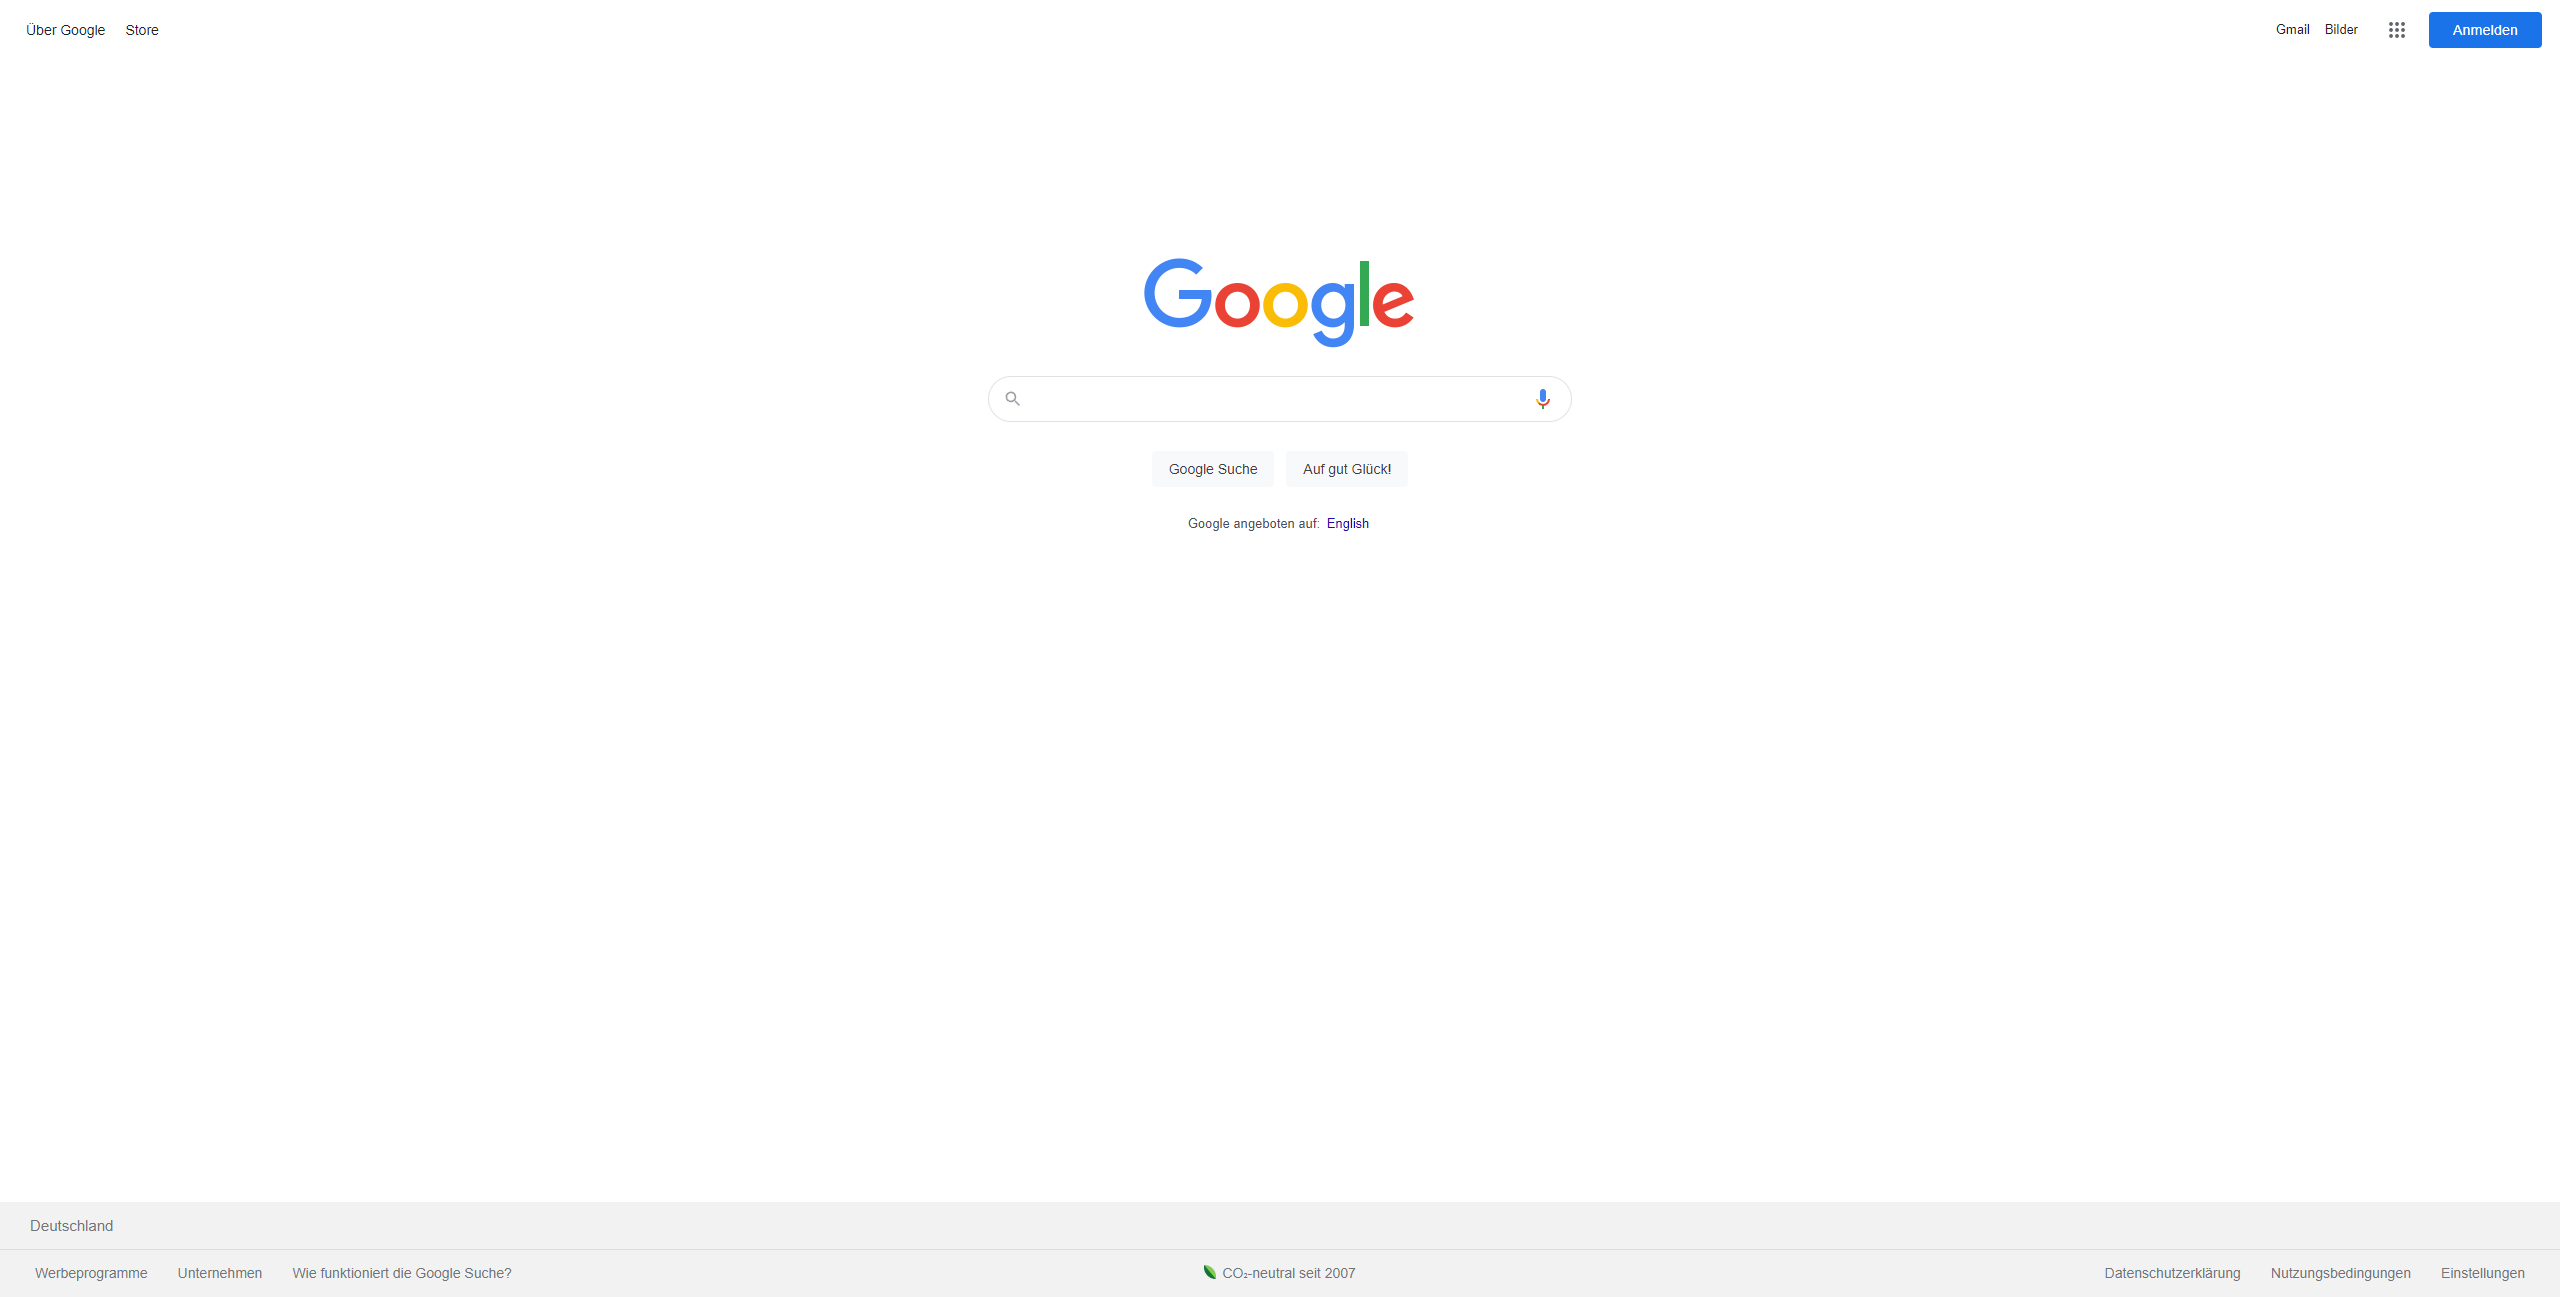
\includegraphics[height=0.3\textheight]{google_home}}\caption{Google Home}\label{fig:google_home}
  \end{figure}
  \begin{figure}[h]
    \centering
    \fbox{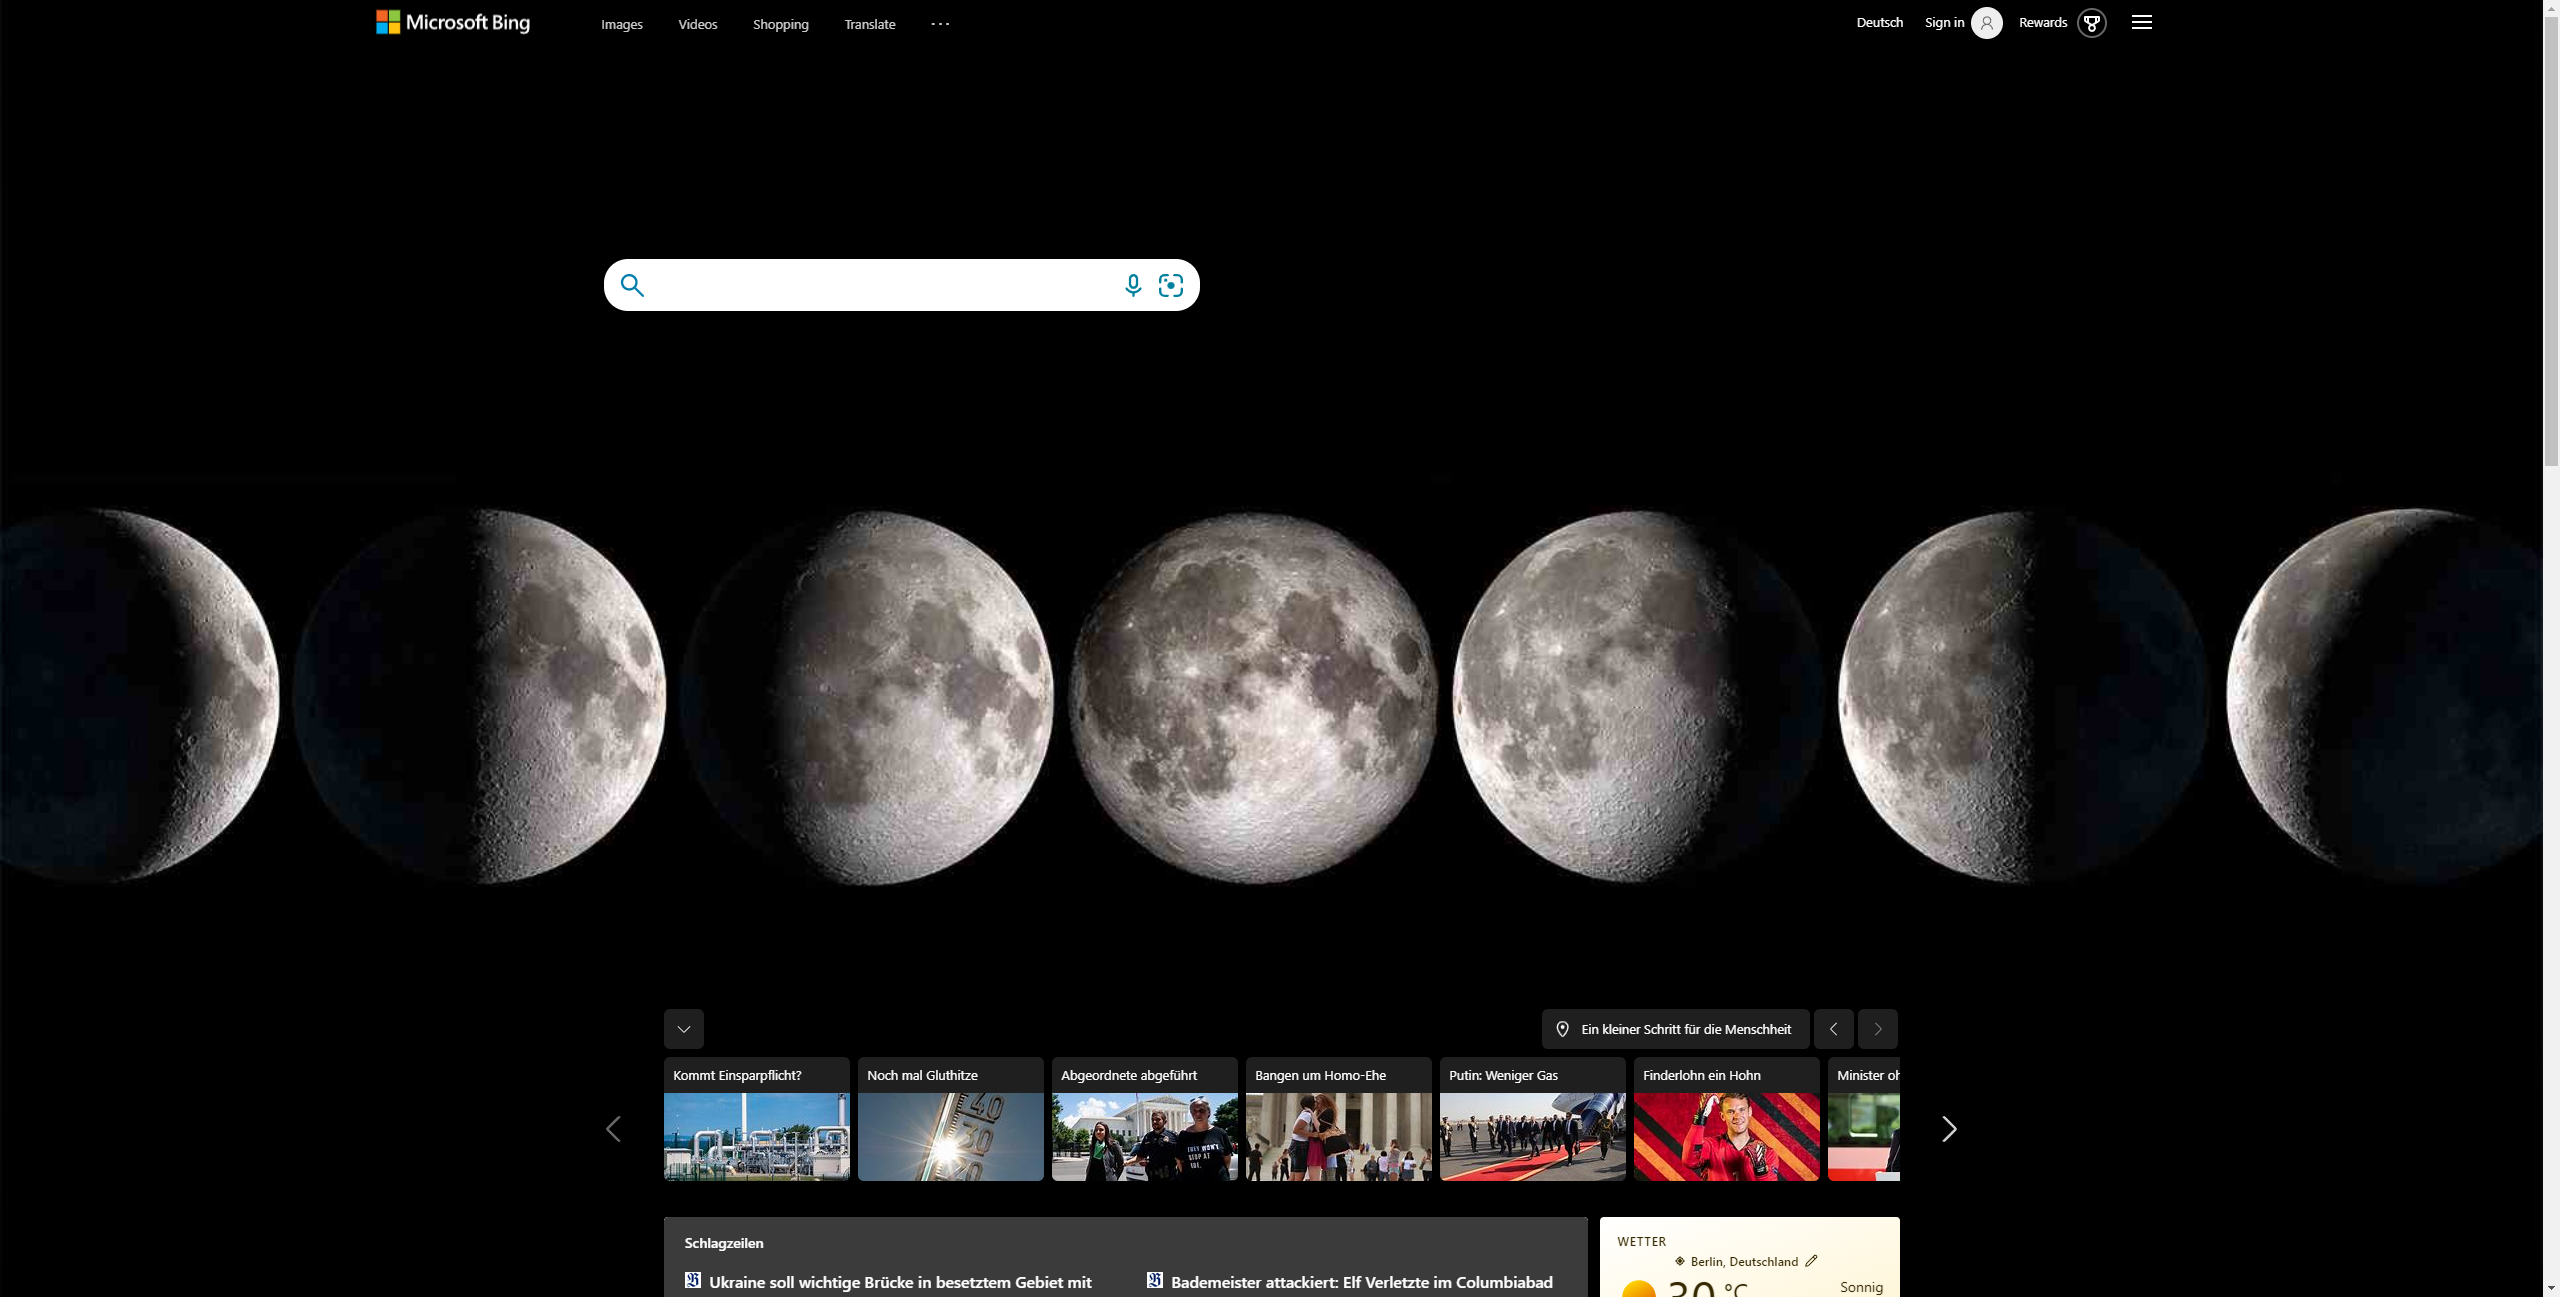
\includegraphics[height=0.3\textheight]{bing_home}}\caption{Bing Home}\label{fig:bing_home}
  \end{figure}
  \begin{figure}[h]
    \centering
    \fbox{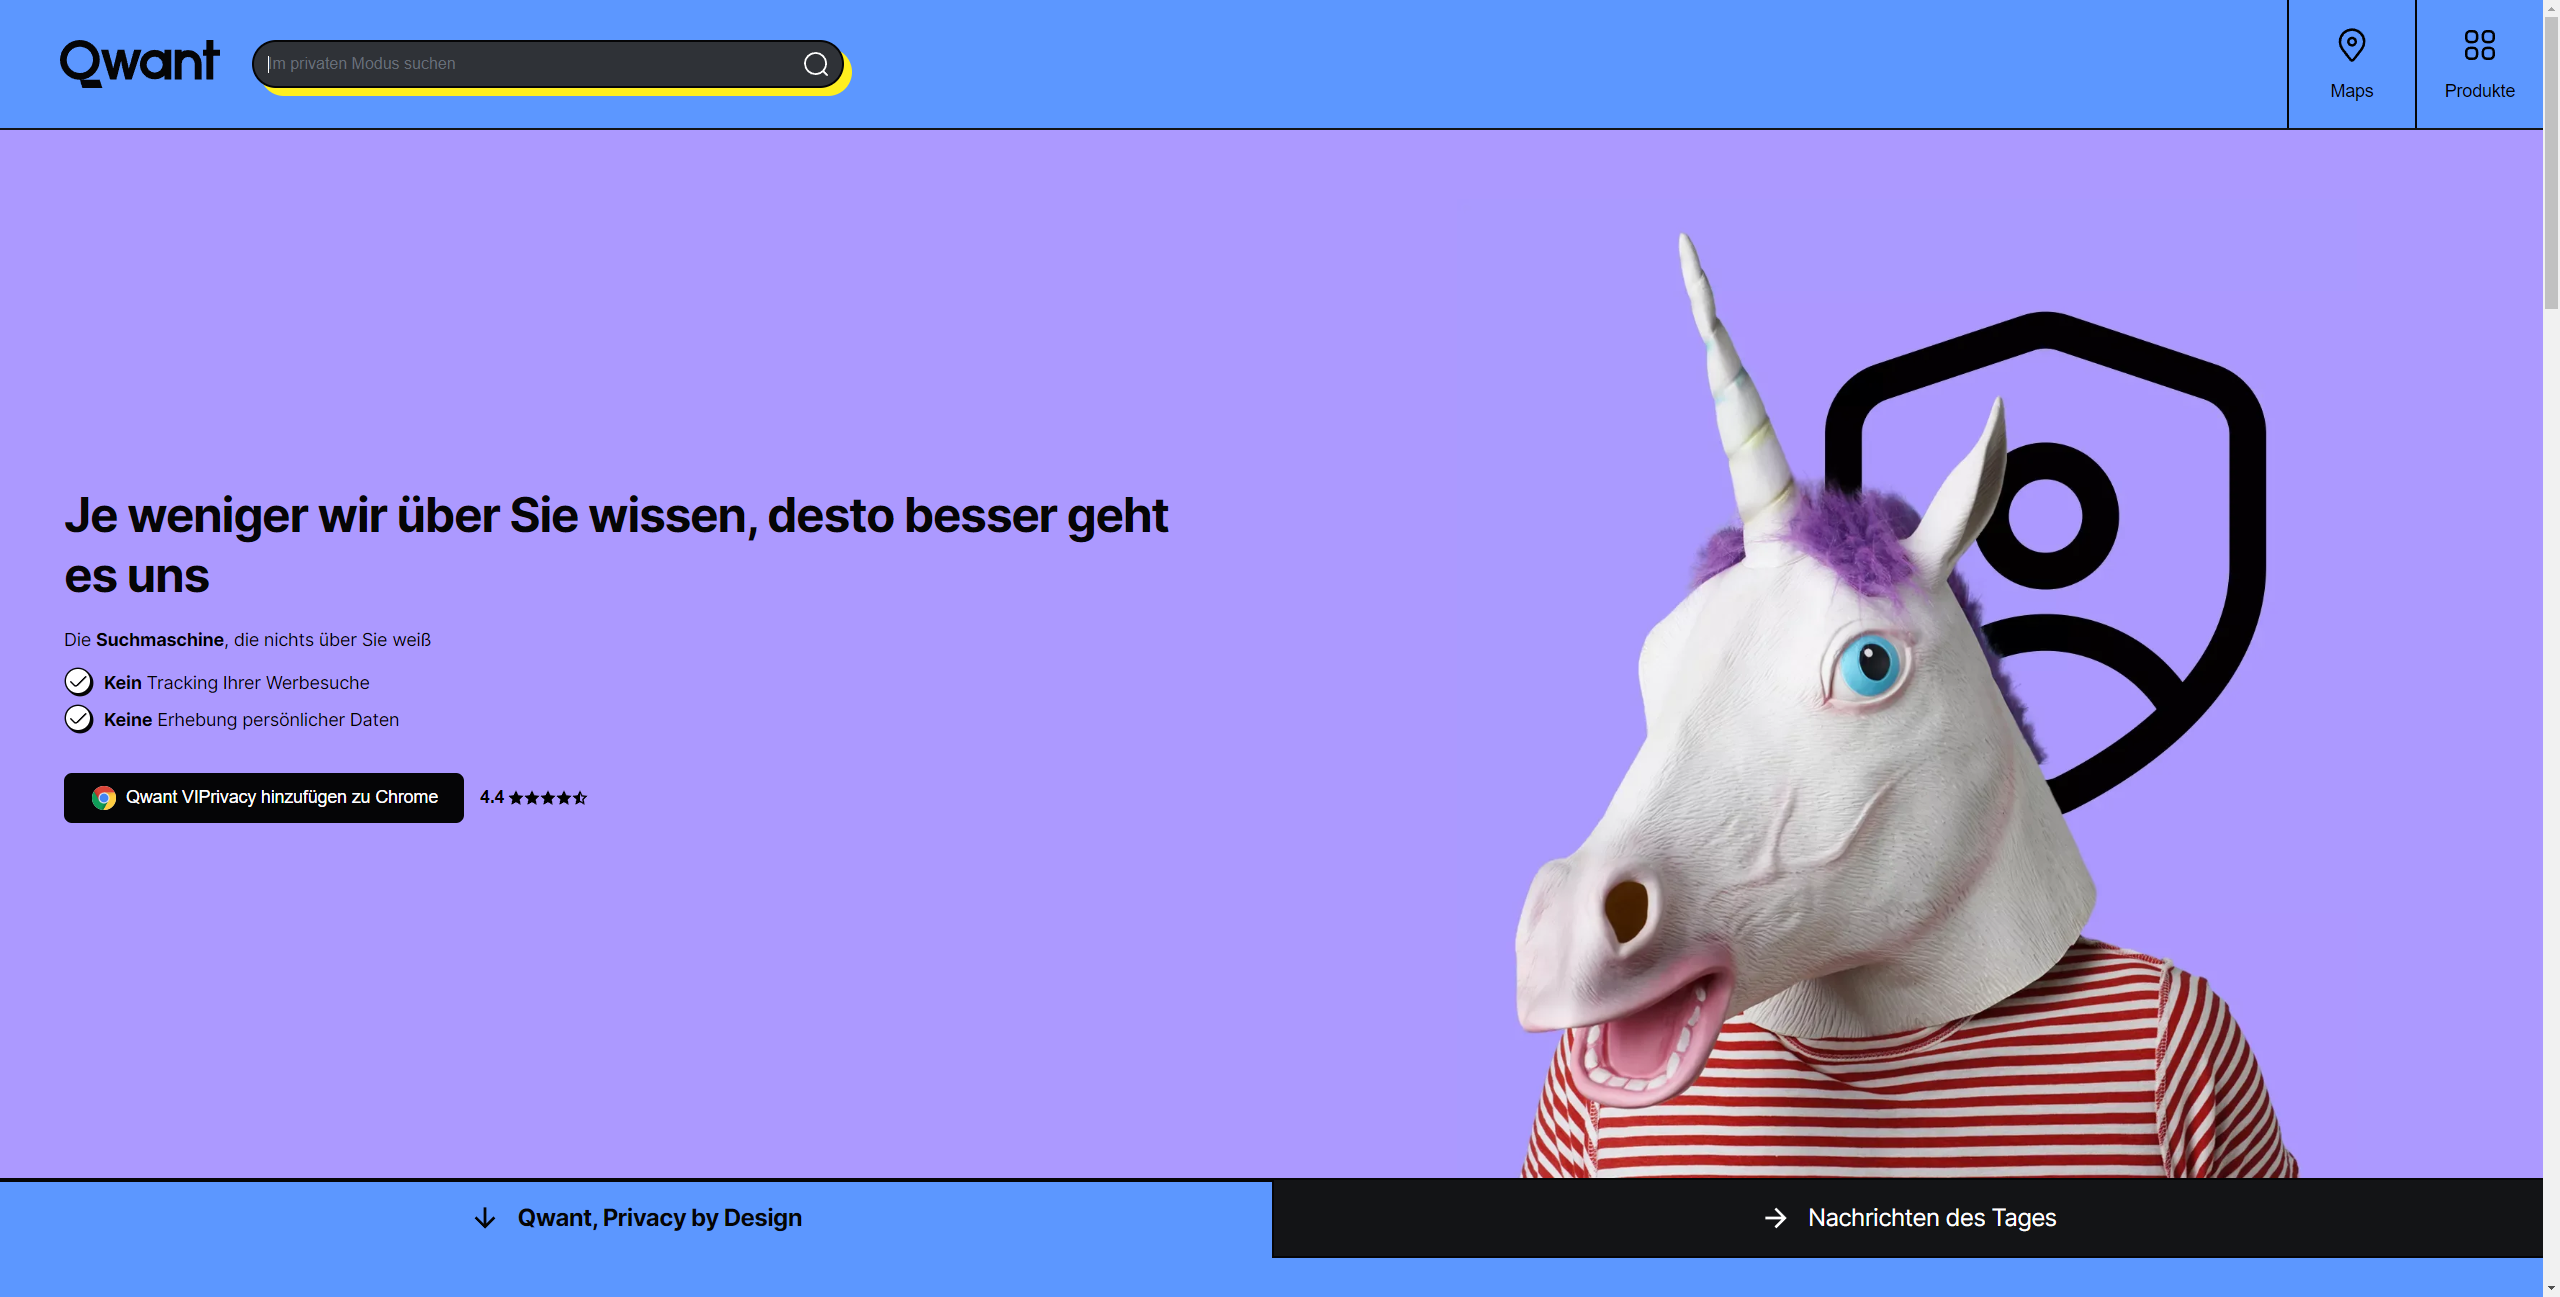
\includegraphics[height=0.3\textheight]{qwant_home}}\caption{Qwant Home}\label{fig:qwant_home}
  \end{figure}
\end{appendix}
\end{document}